\documentclass[11pt]{article}
\usepackage[utf8]{inputenc}
\usepackage[T1]{fontenc}
\usepackage{amsmath}
\usepackage{amsfonts}
\usepackage{amssymb}
\usepackage[version=4]{mhchem}
\usepackage{stmaryrd}
\usepackage{graphicx}
\usepackage[export]{adjustbox}
\graphicspath{ {./images/} }

\begin{document}
\section*{Reading}
Moments of the Distribution: Mean, Variance, Skewness, and Kurtosis

Random variables, such as an asset's return or the timing of uncertain cash flows, can be viewed as forming a probability distribution. Probability distributions have an infinite number of possible shapes, only some of which represent well-known shapes, such as a normal distribution.

The moments of a return distribution are measures that describe the shape of a distribution. As an analogy, in mathematics, researchers often use various parameters to describe the shape of a function, such as its intercept, its slope, and its curvature. Statisticians often use either the raw moments or the central moments of a distribution to describe its shape. Generally, the first four moments are referred to as mean, variance, skewness, and kurtosis. The formulas of these four moments are somewhat similar, differing primarily by the power to which the observations are raised: mean uses the first power, variance squares the terms, skewness cubes the terms, and kurtosis raises the terms to the fourth power.

\section*{The Formulas of the First Four Raw Moments}
Statistical moments can be raw moments or central moments. Further, the moments are sometimes standardized or scaled to provide more intuitive measures, as will be discussed later. We begin with raw moments, discussing the raw moments of an investment's return, $R$. Raw moments have the simplest formulas, wherein each moment is simply the expected value of the variable raised to a particular power:


\begin{equation*}
n \text {th Raw Moment }=\mathrm{E}\left(R^{n}\right) \tag{1}
\end{equation*}


The most common raw moment is the first raw moment and is known as the mean, or expected value, and is an indication of the central tendency of the variable. With $n=1$, Equation 1 is the formula for expected value:


\begin{equation*}
\text { 1st Raw Moment }=\mathrm{E}\left(R^{1}\right)=\mathrm{E}(R) \tag{2}
\end{equation*}


The expected value of a variable is the probability-weighted average of its outcomes:


\begin{equation*}
\mathrm{E}(R)=\sum_{i} \operatorname{prob}_{i} \times R_{i} \tag{3}
\end{equation*}


where prob $_{i}$ is the probability of $R_{i}$.

Equation 3 expresses the first raw moment in terms of probabilities and outcomes. Using historical data, for a sample distribution of $n$ observations, the mean is typically equally weighted and is estimated by the following:


\begin{equation*}
\text { Mean }=\bar{R}=\frac{1}{n} \sum_{i} R_{i} \tag{4}
\end{equation*}


Thus, Equation 4 is a formula for estimating Equation 2 using historical observations. The historical mean is often used as an estimate of the expected value when observations from the past are assumed to be representative of the future. Other raw moments can be generated by inserting a higher integer value for $n$ in Equation 1. But the raw moments for $n>1$ are less useful for our purposes than the highly related central moments.

\section*{The Formulas of Central Moments}
Central moments differ from raw moments because they focus on deviations of the variable from its mean (whereas raw moments are measured relative to zero). Deviations are defined as the value of a variable minus its mean, or expected value. If an observation exceeds its expected value, the deviation is positive by the distance by which it exceeds the expected value. If the observation is less than its expected value, the deviation is a negative number. Each central moment applies the following equation to the deviations:


\begin{equation*}
n \text {th Central Moment }=\mathrm{E}\left[(R-\mu)^{n}\right] \tag{5}
\end{equation*}


where $\mu=$ the expected value of $R$. The term inside the parentheses is the deviation of $R$ from its mean, or expected value. The first central moment is equal to zero by definition, because the expected value of the deviation from the mean is zero. When analysts discuss statistical moments, it is usually understood that the first moment is a raw moment, meaning the mean, or expected value. But the second through fourth moments are usually automatically expressed as central moments because in most applications the moments are more useful when expressed in terms of deviations.

The variance is the second central moment and is the expected value of the deviations squared, providing an indication of the dispersion of a variable around its mean:


\begin{equation*}
\text { 2nd Central Moment }=\text { Variance }=\mathrm{E}\left[(R-\mu)^{2}\right] \tag{6}
\end{equation*}


The variance is the probability weighted average of the deviations squared. By squaring the deviations, any negative signs are removed (i.e., any negative deviation squared is positive), so the variance $[V(R)]$ becomes a measure of dispersion. In the case of probability-weighted outcomes, this can be written as:


\begin{equation*}
V(R)=\sigma^{2}=\sum_{i} \operatorname{prob}_{i} \times\left(R_{i}-\mu\right)^{2} \tag{7}
\end{equation*}


The variance shown in Equation 7 is often estimated with a sample of historical data. For a sample distribution, the variance with equally weighted observations is estimated as:


\begin{equation*}
\text { Variance }=\frac{1}{n-1} \sum_{i}\left(R_{i}-\bar{R}\right)^{2} \tag{8}
\end{equation*}


The mean in Equation $8, \bar{R}$, is usually estimated using the same sample. The use of $n-1$ in the equation (rather than $n$ ) enables a more accurate measure of the variance when the estimate of the expected value of the variable has been computed from the same sample. The square root of the variance is an extremely popular and useful measure of dispersion known as the standard deviation:


\begin{equation*}
\text { Standard Deviation }=\sqrt{\sigma^{2}}=\sigma \tag{9}
\end{equation*}


In investment terminology, volatility is a popular term that is used synonymously with the standard deviation of returns. Other central moments can be generated by inserting a higher integer value for $n$ in Equation 5. But the central moments for $n=3$ (skewness) and $n=4$ (kurtosis) are typically less intuitive and less well-known than their scaled versions. In other words, rather than using the third and fourth central moments, slightly modified formulas are used to generate scaled measures of skewness and kurtosis. These two scaled measures are detailed in the next two sections.

\section*{Skewness}
The third central moment is the expected value of a variable's cubed deviations:


\begin{equation*}
\text { 3rd Central Moment }=\mathrm{E}\left[(R-\mu)^{3}\right] \tag{10}
\end{equation*}


A problem with the third central moment is that it is generally affected by the scale. Thus, a distribution's third central moment for a variable measured in daily returns differs dramatically if the daily returns are expressed as annualized returns. To provide this measure with a more intuitive scale, investment analysts typically use the standardized third moment (the relative skewness or simply the skewness). The skewness is equal to the third central moment divided by the standard deviation of the variable cubed and serves as a measure of asymmetry:


\begin{equation*}
\text { Skewness }=\mathrm{E}\left[(R-\mu)^{3}\right] / \sigma^{3} \tag{11}
\end{equation*}


Skewness is dimensionless, since changes in the scale of the returns affect the numerator and denominator proportionately, leaving the fraction unchanged. By cubing the deviations, the sign of each deviation is retained because a negative value cubed remains negative. Further, cubing the deviations provides a measure of the direction in which the largest deviations occur, since the cubing causes large deviations to be much more influential than the smaller deviations. The result is that the measure of skewness in Equation 11 provides a numerical measure of the extent to which a distribution flares out in one direction or the other. A positive value indicates that the right tail is larger (the mass of the distribution is concentrated on the left side), and a negative value indicates that the left tail is larger (the mass of the distribution is concentrated on the right side). A skewness of zero can result from a symmetrical distribution, such as the normal distribution, or from any other distribution in which the tails otherwise balance out within the equation. The top illustration of the next exhibit depicts negatively skewed, symmetric, and positively skewed distributions.\\
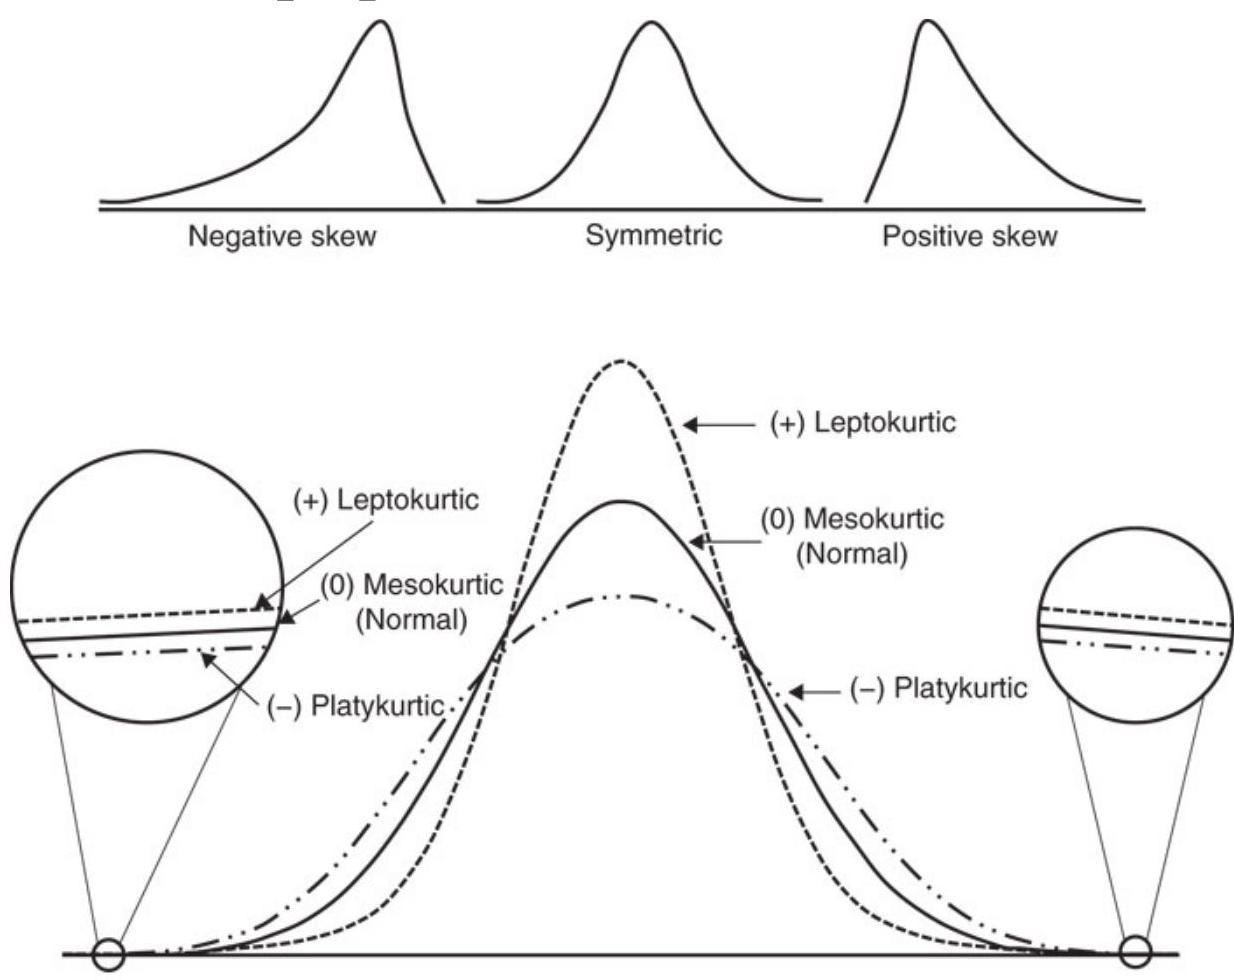
\includegraphics[max width=\textwidth, center]{2024_04_10_817da4f390bf5301abf8g-4(3)}

\begin{center}
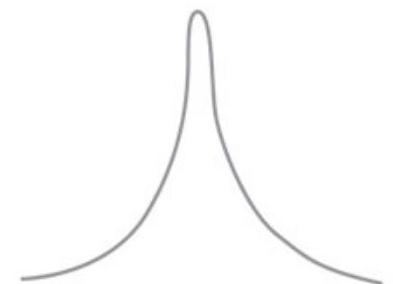
\includegraphics[max width=\textwidth]{2024_04_10_817da4f390bf5301abf8g-4}
\end{center}

Leptokurtic distribution

\begin{center}
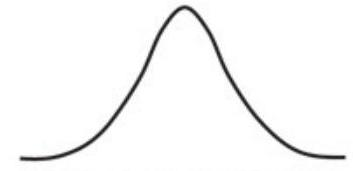
\includegraphics[max width=\textwidth]{2024_04_10_817da4f390bf5301abf8g-4(1)}
\end{center}

Mesokurtic distribution

\begin{center}
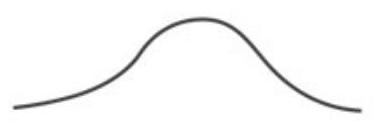
\includegraphics[max width=\textwidth]{2024_04_10_817da4f390bf5301abf8g-4(2)}
\end{center}

Platykurtic distribution

\section*{Skewness and Kurtosis}
\section*{Excess Kurtosis}
The fourth central moment is the expected value of a variable's deviations raised to the fourth power:


\begin{equation*}
\text { 4th Central Moment }=\mathrm{E}\left[(R-\mu)^{4}\right] \tag{12}
\end{equation*}


As with the third central moment, a problem with the fourth central moment is that it is difficult to interpret its magnitude. To provide this measure with a more intuitive scale, investment analysts do two things. First, they divide the moment by the standard deviation of the variable raised to the fourth power (to make it dimensionless):


\begin{equation*}
\text { Kurtosis }=\mathrm{E}\left[(R-\mu)^{4}\right] / \sigma^{4} \tag{13}
\end{equation*}


The resulting measure, known as kurtosis, is shown in Equation 13 and primarily serves as an indicator of the size of the extreme tails of a distribution. In the case of a normally distributed variable, the estimated kurtosis has a value that approaches 3.0 (as the sample size is increased). The second adjustment that analysts often perform to create a more intuitive measure of kurtosis is to subtract 3.0 from the result to derive a measure, known as excess kurtosis. Excess kurtosis provides a more intuitive measure of kurtosis relative to the normal distribution because it has a value of zero in the case of the normal distribution:


\begin{equation*}
\text { Excess Kurtosis }=\left\{\mathrm{E}\left[(R-\mu)^{4}\right] / \sigma^{4}\right\}-3 \tag{14}
\end{equation*}


Since 3.0 is the kurtosis of a normally distributed variable, after subtracting 3.0 from the kurtosis, a positive excess kurtosis signals a level of kurtosis that is higher than observed in a normally distributed variable, an excess kurtosis of 0.0 indicates a level of kurtosis similar to that of a normally distributed variable, and a negative excess kurtosis signals a level of kurtosis that is lower than that observed in a normally distributed variable.

Kurtosis is typically viewed as capturing the fatness of the tails of a distribution, with high values of kurtosis (or positive values of excess kurtosis) indicating fatter tails (i.e., higher probabilities of extreme outcomes) than are found in the case of a normally distributed variable.

In summary, the mean, variance, skewness, and kurtosis of a return distribution indicate the location and shape of a distribution, and are often a key part of measuring and communicating the risks and rewards of various investments. Familiarity with each can be a critical component of a high-level understanding of the analysis of alternative investments.

\section*{Platykurtosis, Mesokurtosis, and Leptokurtosis}
The level of kurtosis is sufficiently important in analyzing alternative investment returns that the statistical descriptions of the degree of kurtosis and the related terms have become industry standards. If a return distribution has no excess kurtosis, meaning it has the same kurtosis as the normal distribution, it is said to be mesokurtic, mesokurtotic, or normal tailed, and to exhibit mesokurtosis. The tails of the distribution would have the same magnitude as the normal distribution.

The middle illustration in the Skewness and Kurtosis exhibit above depicts that kurtosis can be viewed by the fatness of the tails of a distribution. If a return distribution has negative excess kurtosis, meaning less kurtosis than the normal distribution, it is said to be platykurtic, platykurtotic, or thin tailed, and to exhibit platykurtosis. If a return distribution has positive excess kurtosis, meaning it has more kurtosis than the normal distribution, it is said to be leptokurtic, leptokurtotic, or fat tailed, and to exhibit leptokurtosis.

The bottom illustration in the Skewness and Kurtosis exhibit depicts leptokurtic, mesokurtic, and platykurtic distributions. A leptokurtic distribution (positive excess kurtosis) with fat tails is illustrated on the left. A platykurtic distribution (negative excess kurtosis) with thin tails and a rounded center is illustrated on the right. In the middle is a normal mesokurtic distribution (no excess kurtosis). The key to recognizing excess kurtosis visually is comparing the thickness of the tails of both sides of the distribution relative to the tails of a normal distribution.


\end{document}